\documentclass[11pt,compress,t,notes=noshow, aspectratio=169, xcolor=table]{beamer}

\usepackage{../../style/lmu-lecture}
% Defines macros and environments
% This file is included in slides and exercises

% Rarely used fontstyle for R packages, used only in 
% - forests/slides-forests-benchmark.tex
% - exercises/single-exercises/methods_l_1.Rnw
% - slides/cart/attic/slides_extra_trees.Rnw
\newcommand{\pkg}[1]{{\fontseries{b}\selectfont #1}}

% Spacing helpers, used often (mostly in exercises for \dlz)
\newcommand{\lz}{\vspace{0.5cm}} % vertical space (used often in slides)
\newcommand{\dlz}{\vspace{1cm}}  % double vertical space (used often in exercises, never in slides)
\newcommand{\oneliner}[1] % Oneliner for important statements, used e.g. in iml, algods
{\begin{block}{}\begin{center}\begin{Large}#1\end{Large}\end{center}\end{block}}

% Don't know if this is used or needed, remove?
% textcolor that works in mathmode
% https://tex.stackexchange.com/a/261480
% Used e.g. in forests/slides-forests-bagging.tex
% [...] \textcolor{blue}{\tfrac{1}{M}\sum^M_{m} [...]
% \makeatletter
% \renewcommand*{\@textcolor}[3]{%
%   \protect\leavevmode
%   \begingroup
%     \color#1{#2}#3%
%   \endgroup
% }
% \makeatother


\title{Interpretable Machine Learning}
% \author{LMU}
%\institute{\href{https://compstat-lmu.github.io/lecture_iml/}{compstat-lmu.github.io/lecture\_iml}}
\date{}

\begin{document} 

\newcommand{\titlefigure}{figure/whitebox}
\newcommand{\learninggoals}{
%\item What characteristics does an interpretable model have?
\item Why should we use interpretable models?
\item Advantages and disadvantages of interpretable models
}

\lecturechapter{Inherently Interpretable Models - Motivation}
\lecture{Interpretable Machine Learning}

\begin{frame}{Motivation}
%Achieving interpretability by using interpretable models is the most straightforward approach
%\bigskip
\begin{columns}[T, totalwidth = \textwidth]
    \begin{column}{0.58\textwidth}
    \begin{itemize}
        %\item Obtaining interpretations by using interpretable models is the easiest and least error-prone approach
       \item Achieving interpretability by using interpretable models is the most straightforward approach
         \item Classes of models deemed interpretable:
   \begin{itemize}
  \footnotesize
  \item (Generalized) linear models (LM, GLM)
  \item Generalized additive models (GAM)
  \item Decision trees
  \item Rule-based learning
  \item Model-based / component-wise boosting
  \item ...
\end{itemize}
    \end{itemize}
    

    \end{column}
    \begin{column}{0.42\textwidth}  %%<--- here
    \centering
  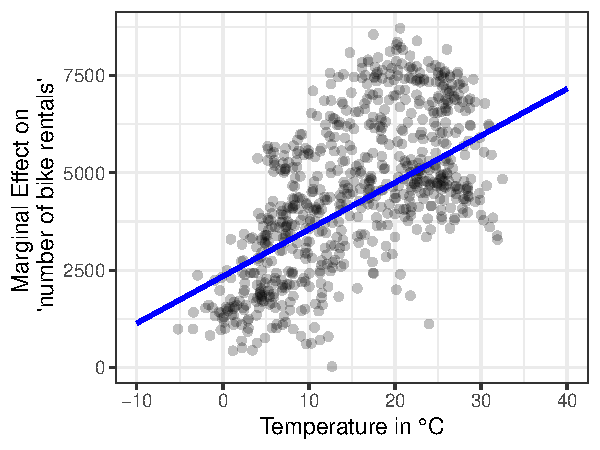
\includegraphics[width = 0.8\textwidth]{figure/main_effect_lm_temp.pdf}
  \begin{center}
    $\leadsto$ LM provides straightforward interpretation
  \end{center}

    \end{column}
\end{columns}

\begin{itemize}
 \item Often there is a trade-off between interpretability and model performance 
        %(but not always)
\end{itemize}
\centering
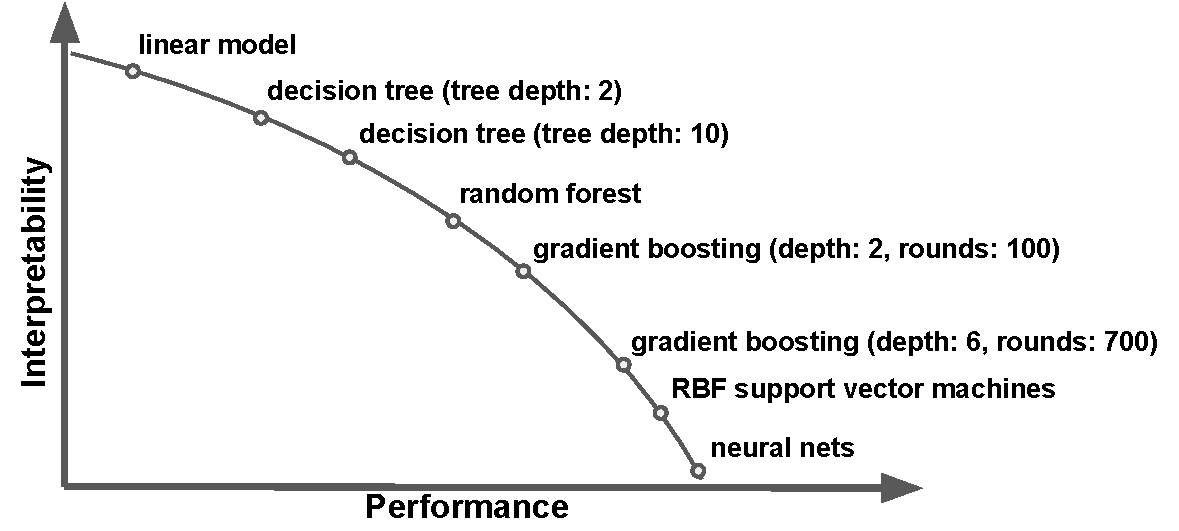
\includegraphics[width=0.55\textwidth]{figure/performance_vs_interpretability.pdf}
    % Quelle: https://docs.google.com/presentation/d/12ZPrTjBKEUT-7drdyUJCQGK0oHVDtYIVd2_6byE62f0/edit?usp=sharing
\end{frame}

\begin{frame}{Advantages}
\begin{columns}[T, totalwidth=\textwidth]
\begin{column}{0.75\textwidth}
    \begin{itemize}[<+->]
    \itemsep1em
        \item Interpretable models are transparent by design, making many model-agnostic explanation methods unnecessary\\
        %For inherently interpretable models some additional model-agnostic interpretation methods not required \\
        $\leadsto$ Eliminates an extra source of estimation error
        \item They often have few hyperparameters and are structurally simple (e.g., linear, additive, sparse, monotonic)\\
$\leadsto$ Easy to train, fast to tune, and straightforward to explain
        % \item Interpretable models often simple \\
        % $\leadsto$ training time is fairly small
        % \item Some interpretable models estimate monotonic effects \\
        % %the monotonicity constraint \\
        % $\leadsto$ Simple to explain as larger feature values always lead to higher (or smaller) outcomes (e.g., GLMs)
        \item Many people are familiar with simple interpretable models \\
        $\leadsto$ Increases trust, facilitates communication of results
        %\item Implementations are available in many programming languages \\
        %$\leadsto$ Simple models are easier to deploy in practice or implement from scratch
    \end{itemize}
\end{column}
\begin{column}{0.25\textwidth}
    \begin{center}
        \begin{tikzpicture}[scale=0.6, transform shape]
        \usetikzlibrary{arrows}
            \usetikzlibrary{shapes}
            \tikzset{treenode/.style={draw, circle, font=\small}}
            \tikzset{line/.style={draw, thick}}
            \node [treenode, draw=red] (a0) {$a_0$};
            \node [treenode, below=0.75cm of a0, xshift=-1cm]  (a1) {$a_1$};
            \node [treenode, draw=red, below=0.75cm of a0, xshift=1cm]  (a2) {$a_2$};
     
            \node [treenode, draw=red, below=0.75cm of a2, xshift=-1cm] (a3) {$a_3$};
            \node [treenode, below=0.75cm of a2, xshift=1cm]  (a4) {$a_4$};
     
            \node [treenode, below=0.75cm of a3, xshift=-1cm] (a5) {$a_5$};
            \node [treenode, below=0.75cm of a3, xshift=1cm]  (a6) {$a_6$};
     
            \path [line] (a0.south) -- + (0,-0.4cm) -| (a1.north) node [midway, above] {$x_1<0.3$};
            \path [line] (a0.south) -- +(0,-0.4cm) -|  (a2.north) node [midway, above] {$x_1\geq0.3$};
     
            \path [line] (a2.south) -- + (0,-0.4cm) -| (a3.north) node [midway, above] {$x_1<0.6$};;
            \path [line] (a2.south) -- +(0,-0.4cm) -|  (a4.north) node [midway, above] {$x_1\geq0.6$};
     
          
            \path [line] (a3.south) -- + (0,-0.4cm) -| (a5.north) node [midway, above] {$x_2<0.2$};;
            \path [line] (a3.south) -- +(0,-0.4cm) -|  (a6.north) node [midway, above] {$x_2\geq0.2$};
     
        \end{tikzpicture}
        
        \vspace{0.5cm}
        
        \includegraphics<2->[width = \textwidth]{figure/main_effect_lm_temp.pdf}
    \end{center}
\end{column}
\end{columns}
\end{frame}

\begin{frame}{Disadvantages \& Limitations}
\begin{columns}[totalwidth=\textwidth]
\begin{column}{0.75\textwidth}
    \begin{itemize}%[<+->]
    \itemsep1em
        \item<1-> Often require assumptions about data / model structure \\%Often certain assumptions about data / model structure required\\
        $\leadsto$ If assumptions are wrong, models may perform bad 
        %\item In high-dimensional settings, it may not be feasible to find and define all feature relationships
        %\item If the wrong assumptions are made, interpretable models may have a bad predictive performance
        %\pause
        \item<2-> Interpretable models may also be hard to interpret, e.g.:
    \begin{itemize}
        \item LM with lots of features and interactions 
        \item Decision trees with huge tree depth
    \end{itemize}
    \end{itemize}
\end{column}
\begin{column}{0.25\textwidth}
    \begin{center}
        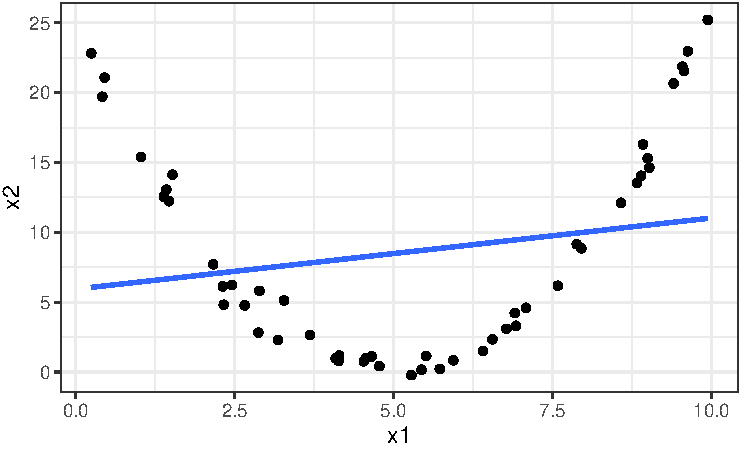
\includegraphics[width = \textwidth]{figure/lm_bad_fit.pdf} 
    \end{center}
\end{column}
\end{columns}
\quad \\

\begin{itemize}
\itemsep1em
        \item<3-> 
        %No automatic modeling of complex relationships due to limited model flexibility
        Often do not automatically model complex relationships due to limited flexibility
        \\
        e.g., high-order main or interaction effects need to be specified manually in an LM

        %\pause
     \item<4-> Inherently interpretable models do not address all explanation needs\\
$\leadsto$ Complementary model-agnostic methods (e.g., counterfactuals) remain valuable for specific tasks
     % Inherently interpretable models do not provide all types of explanations
     % %% one might be interested
     % \\
     % $\leadsto$ Methods providing other types of explanations still useful  (e.g., counterfactual explanations)
     %Methods providing other types of explanations still useful  (e.g., counterfactual explanations)
     %Still requires application of model-agnostic interpretation techniques if certain types of explanations are of interest (e.g., counterfactual explanations)
\end{itemize}
\end{frame}

\begin{frame}{Further Comments}

    \begin{itemize}
    %\itemsep1em
        \item<1-> Some researchers advocate for inherently interpretable models instead of explaining black boxes after training \citebutton{Rudin 2019}{https://www.nature.com/articles/s42256-019-0048-x}
        \begin{itemize}
        \item Built-in interpretation $\Rightarrow$ fewer risks from misleading post-hoc explanations
        
            %\item \ldots instead of explaining uninterpretable models post-hoc
            % \item Can sometimes work out by spending enough time and energy on data pre-processing or manual feature engineering
            \item  Good performance possible with effort on preprocessing / feat. engineering
    \item But interpretability depends on meaning of created features\\
    $\leadsto$ E.g., PCA keeps models linear, but yields hard-to-interpret components
            %, or data cleaning
        \end{itemize}
        %\pause
        %\footnote[frame]{Rudin, C. Stop explaining black box machine learning models for high stakes decisions and use interpretable models instead. Nat Mach Intell 1, 206–215 (2019).}
        % {https://www.nature.com/articles/s42256-019-0048-x}
       %\item Interpretable models also have the potential for a high predictive performance, but require more knowledge and time spent on data preprocessing
       % \item<2->[$\leadsto$] Drawback: Hard to achieve for data for which end-to-end learning is crucial\\ 
       % $\leadsto$ e.g., hard to extract good features for image / text data\\ 
       % $\leadsto$ information loss can lead to bad performance
      \item<2-> Limitation: Less suited for complex data where end-to-end learning is crucial
\begin{itemize}
    \item Applies to image, text, or sensor data where features must be learned %from raw input
    \item Manual extraction of interpretable features is difficult \\$\Rightarrow$ Information loss and lower performance
\end{itemize}
       %(e.g., for image / text data extraction of good features is hard $\leadsto$ information loss = bad performance)
       %(e.g., image and text data would require good feature extraction steps $\leadsto$ information loss)
        %\pause
        %\item One can assume a trade-off between interpretability and model performance which generally (but not always) holds
        %\item<3-> Often there is a trade-off between interpretability and model performance 
        %(but not always)
    \end{itemize}
    
    %\smallskip
    
    %\only<3>{\centering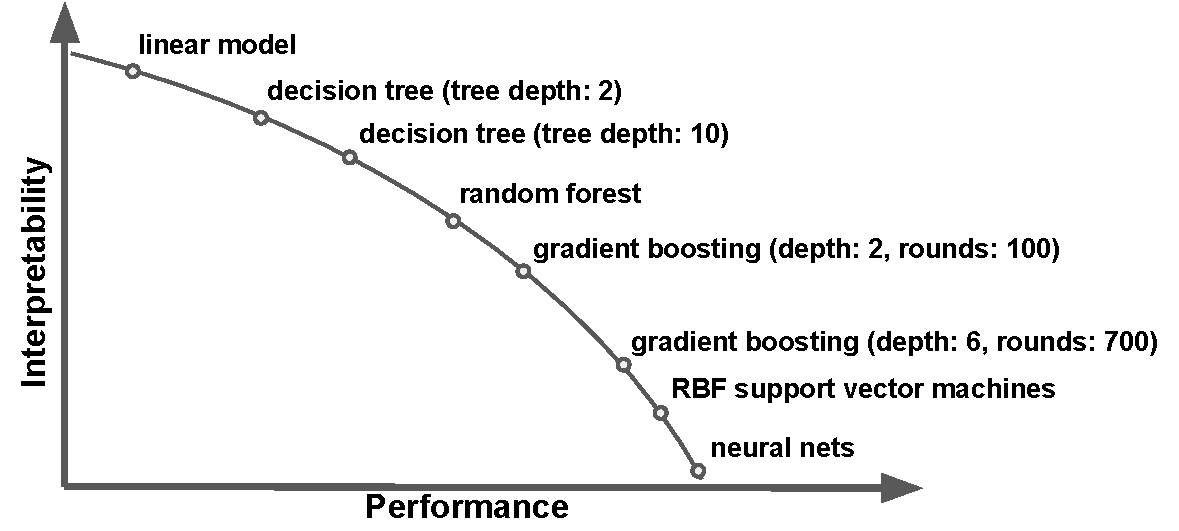
\includegraphics[width=0.65\textwidth]{figure/performance_vs_interpretability.pdf}}
    % Quelle: https://docs.google.com/presentation/d/12ZPrTjBKEUT-7drdyUJCQGK0oHVDtYIVd2_6byE62f0/edit?usp=sharing

\end{frame}


\begin{frame}{Recommendation}
    % \begin{itemize}
    %     \item Start with most simple model that makes sense for application at hand
    %     \item Gradually increase complexity if performance is insufficient\\
    %     $\leadsto$ will usually lower interpretability and require additional interpretation methods
    %     \item Choose the most simple, sufficient model (Occam's razor)
    % \end{itemize} 
\begin{itemize}
    \item Begin with the simplest model appropriate for the task
    \item Increase complexity only if necessary to meet performance requirements\\
    $\leadsto$ Typically reduces interpretability and requires model-agnostic explanations
    \item Choose the simplest model with sufficient accuracy 
    $\leadsto$ Occam’s razor
\end{itemize}
    \bigskip

% \begin{columns}[T, totalwidth=\textwidth]
% \begin{column}{0.5\textwidth}
% \centering \textbf{Bike Data}
%     \begin{table}[ht]
%         \centering
%         \begin{tabular}{lrr}
%             \hline
%             Model & RMSE & $R^2$ \\ 
%             \hline
%             LM & 142.39 & 0.38 \\ 
%             Tree & 98.71 & 0.70 \\ 
%             Random Forest & 57.07 & 0.90 \\ 
%             Boosting & 197.42 & -0.18 \\  
%             \hline
%         \end{tabular}
%     \end{table}
% \end{column}
% \begin{column}{0.5\textwidth}
% \centering \textbf{Boston Housing Data}
%     \begin{table}[ht]
%         \centering
%         \begin{tabular}{lrr}
%             \hline
%             Model & RMSE & $R^2$ \\ 
%             \hline
%             LM & 0.43 & 1.00 \\ 
%             Tree & 1.81 & 0.96 \\ 
%             Random Forest & 1.77 & 0.96 \\ 
%             Boosting & 16.89 & -2.43 \\
%             \hline
%         \end{tabular}
%     \end{table}
% \end{column}
% \end{columns}
% code for tables in rsrc/tab_ml_comparison.R

\centering \textbf{Bike Data, 4-fold CV}
\begin{table}[ht]
\centering
\begin{tabular}{lrr}
  \hline
Model & RMSE & $R^2$ \\ 
  \hline
  LM & 800.15 & 0.83 \\ 
  Tree & 981.83 & 0.74 \\ 
  Random Forest & 653.25 & 0.88 \\ 
  Boosting (tuned) & 638.42 & 0.89 \\ 
   \hline
\end{tabular}
\end{table}
\end{frame}



\endlecture
\end{document}
